\documentclass[10pt,a4paper]{article}
\usepackage[margin=2cm]{geometry}
\usepackage[T1]{fontenc}
\usepackage{lmodern}
\usepackage{amsmath,amssymb}
\usepackage{booktabs,tabularx,array}
\usepackage{xcolor}
\usepackage{enumitem}
\usepackage{tikz}
\usetikzlibrary{positioning,arrows.meta,shapes.geometric,fit,calc,backgrounds,shadows,decorations.pathreplacing}
\usepackage[colorlinks=true,linkcolor=blue!50!black,urlcolor=blue!50!black]{hyperref}
\setlist{itemsep=1pt,topsep=2pt}
\setlength{\parskip}{3pt}
\setlength{\parindent}{0pt}

% ---------- colours and styles (same as model_structure.tex) ----------
\definecolor{ro}{HTML}{E6E8EB}
\definecolor{ex}{HTML}{DCEBFB}
\definecolor{lp}{HTML}{FCE3D5}
\definecolor{dat}{HTML}{E2F2DF}
\definecolor{drv}{HTML}{F3E6FA}
\definecolor{ink}{HTML}{1F2328}
\definecolor{accent}{HTML}{2A78D6}
\definecolor{warn}{HTML}{C2410C}
\definecolor{good}{HTML}{1E8E3E}
\definecolor{chg}{HTML}{EB6834}

\tikzset{
  box/.style={draw=ink!70, rounded corners=2pt, align=center, font=\small, inner sep=4pt, minimum height=7mm},
  datbox/.style={box, fill=dat},
  lpbox/.style={box, fill=lp},
  arr/.style={-{Stealth[length=2.2mm]}, thick, ink!75},
  darr/.style={-{Stealth[length=2.2mm]}, thick, dashed, ink!55},
  lab/.style={font=\scriptsize\itshape, text=ink!70, fill=white, inner sep=1pt},
}

\newcommand{\code}[1]{\texttt{#1}}
\newcommand{\lamstar}{\lambda^{\star}}
\newcommand{\lamhat}{\hat\lambda}
\newcommand{\R}{\mathcal R}

\title{\textbf{Shaping the battery's bid curves from the multiplier ranges}\\[2pt]
\large A proposal for discussion: what it can fix, what it cannot, and how to test it}
\author{Companion to \code{model\_structure.pdf} (\S7, the multiplier polyhedron)\\and \code{regimes\_design.pdf}\\
\small Status: idea and diagnosis only; nothing implemented}
\date{2026-10-28}

\begin{document}
\maketitle
\vspace{-6mm}

\begin{center}
\fbox{\begin{minipage}{0.93\textwidth}\small
\textbf{In short.} The ranges of valid $\pi_t$ are information the current bid throws away, so turning them into
richer bid curves is worth exploring. But a close look at the loss at \emph{perfect} prices (6.32\% of $V$)
shows it is an \textbf{inter-temporal} problem: an hourly market cannot make a sale at 04--08h conditional on a
purchase at 00--04h, and no price inside the polyhedron changes that. Hourly curves are therefore likely to
help against \textbf{forecast uncertainty} (wrong prices), not against this coordination loss. The ranges fit
most naturally into \textbf{SOC-dependent bids}, an intermediate design between today's hourly curves and
Baldick's SOC-based clearing. Below: the diagnosis, five ideas, the hypotheses each one makes, and a test plan.
\end{minipage}}
\end{center}

\tableofcontents
\clearpage

% =====================================================================
\section{Where the loss at perfect prices comes from}
% =====================================================================

\code{B\_star\_p} bids from the \emph{true} prices $\lamstar$, with the battery's own plan (its self-schedule)
as quantity. It still loses 6.32\% of $V$. Hour by hour (MW; day-ahead = what the market accepted):

\begin{center}\small
\begin{tabular}{@{}lcccccc@{}}
\toprule
interval & 00--04 & 04--08 & 08--12 & 12--16 & 16--20 & 20--24 \\
true price $\lamstar$ (\$/MWh) & 43.1 & 50 & 0 & 0 & 50 & 50 \\
\midrule
Baldick (benchmark) & buy 100 & \textbf{sell 90} & buy 200 & buy 22 & sell 175 & sell 25 \\
battery's plan (self-schedule) & -- & -- & -- & buy 222 & sell 200 & -- \\
\code{B\_star\_p}, day-ahead & buy 100 & \textbf{sell 0} & -- & buy 200 & sell 175 & -- \\
SOC if delivered (MWh) & 360 & 360 & 360 & \textcolor{warn}{\textbf{1\,080}} & 380 & 380 \\
real time & buy 100 & -- & \textcolor{warn}{sell 70} & buy 200 & sell 175 & -- \\
thermal output, real time & 0 & \textbf{100} & 0 & 0 & 0 & \textbf{100} \\
thermal output, Baldick & 0 & 10 & 0 & 0 & 0 & 75 \\
\bottomrule
\end{tabular}
\end{center}

\begin{center}
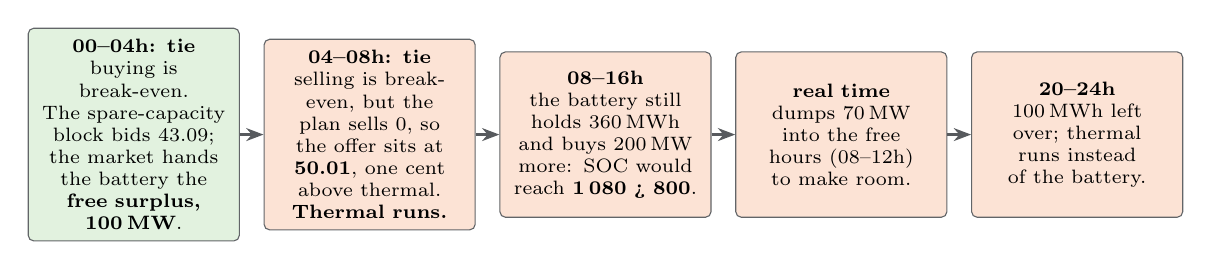
\begin{tikzpicture}[node distance=4mm and 3mm,
  st/.style={box, text width=24mm, minimum height=21mm, font=\scriptsize}]
  \node[st, fill=dat] (a) {\textbf{00--04h: tie}\\buying is break-even.\\The spare-capacity block bids 43.09; the market hands the battery the \textbf{free surplus, 100\,MW}.};
  \node[st, fill=lp, right=of a] (b) {\textbf{04--08h: tie}\\selling is break-even, but the plan sells 0, so the offer sits at \textbf{50.01}, one cent above thermal.\\\textbf{Thermal runs.}};
  \node[st, fill=lp, right=of b] (c) {\textbf{08--16h}\\the battery still holds 360\,MWh and buys 200\,MW more: SOC would reach \textbf{1\,080 > 800}.};
  \node[st, fill=lp, right=of c] (d) {\textbf{real time}\\dumps 70\,MW into the free hours (08--12h) to make room.};
  \node[st, fill=lp, right=of d] (e) {\textbf{20--24h}\\100\,MWh left over; thermal runs instead of the battery.};
  \foreach \x/\y in {a/b, b/c, c/d, d/e} \draw[arr] (\x) -- (\y);
\end{tikzpicture}
\end{center}

\textbf{The cost, item by item} (against Baldick): extra thermal generation $+23\,000$\,\$ (04--08h and
20--24h), redispatch premium $+2\,800$\,\$, less degradation $-269$\,\$, value of the 100\,MWh left at the
end $-4\,000$\,\$: in total $21\,531$\,\$ $=6.32\%$ of $V$.

\textbf{Diagnosis.} Buying at 00--04h and selling at 04--08h belong together: each alone is worth nothing to
the battery, together they save 90\,MW of thermal at 04--08h. The hourly market resolves the two ties
\emph{independently}: the first in favour of buying (the battery is the only bidder for the free surplus), the
second against selling (thermal at 50 beats the offer at 50.01). Baldick's clearing sees both hours and the
SOC at once and resolves them together.

% =====================================================================
\section{What a curve can and cannot express}
% =====================================================================

\begin{center}
\begin{minipage}[t]{0.47\textwidth}
\centering
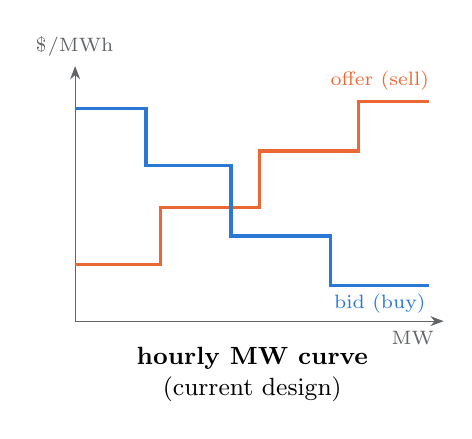
\begin{tikzpicture}[scale=0.9]
  \draw[-{Stealth}, ink!70] (0,0) -- (5.2,0) node[below left, font=\scriptsize]{MW};
  \draw[-{Stealth}, ink!70] (0,0) -- (0,3.6) node[above, font=\scriptsize]{\$/MWh};
  \draw[very thick, chg] (0,0.8) -- (1.2,0.8) -- (1.2,1.6) -- (2.6,1.6) -- (2.6,2.4) -- (4.0,2.4) -- (4.0,3.1) -- (5,3.1);
  \draw[very thick, accent] (0,3.0) -- (1.0,3.0) -- (1.0,2.2) -- (2.2,2.2) -- (2.2,1.2) -- (3.6,1.2) -- (3.6,0.5) -- (5,0.5);
  \node[font=\scriptsize, text=chg] at (4.3,3.4) {offer (sell)};
  \node[font=\scriptsize, text=accent] at (4.3,0.25) {bid (buy)};
  \node[font=\small, align=center] at (2.5,-0.75) {\textbf{hourly MW curve}\\(current design)};
\end{tikzpicture}\\[2pt]
{\small One curve per hour: ``how much at which price, \emph{in this hour}''. It cannot say ``sell at 04--08h
\emph{only if} you bought at 00--04h''.}
\end{minipage}\hfill
\begin{minipage}[t]{0.47\textwidth}
\centering
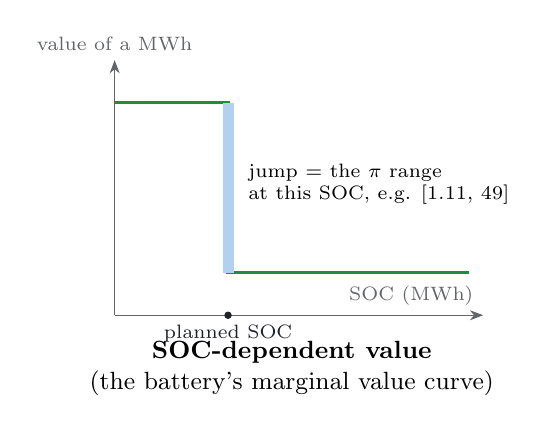
\begin{tikzpicture}[scale=0.9]
  \draw[-{Stealth}, ink!70] (0,0) -- (5.2,0) node[above left, font=\scriptsize]{SOC (MWh)};
  \draw[-{Stealth}, ink!70] (0,0) -- (0,3.6) node[above, font=\scriptsize]{value of a MWh};
  \draw[very thick, good] (0,3.0) -- (1.6,3.0) -- (1.6,0.6) -- (5,0.6);
  \draw[line width=4pt, accent!35] (1.6,0.6) -- (1.6,3.0);
  \node[font=\scriptsize, align=left, anchor=west] at (1.75,1.85) {jump = the $\pi$ range\\at this SOC, e.g. $[1.11,\,49]$};
  \fill[ink] (1.6,0) circle (1.5pt) node[below, font=\scriptsize]{planned SOC};
  \node[font=\small, align=center] at (2.5,-0.75) {\textbf{SOC-dependent value}\\(the battery's marginal value curve)};
\end{tikzpicture}\\[2pt]
{\small The value of a stored MWh as a function of SOC. The $\pi$ range is the vertical jump at the planned SOC.
If the \emph{market} tracks SOC, this curve answers ``sell at 04--08h because you are now full''.}
\end{minipage}
\end{center}

\textbf{Two consequences.}
\begin{enumerate}
  \item \textbf{Choosing inside the range does not fix the coordination loss.} The polyhedron is built around the
    battery's \emph{plan}. Where the plan does not sell (04--08h), every point of $\Pi$ has an offer at or above
    the price, $c_2\ge\lamstar_2=50$. Any curve that stays inside $\Pi$ inherits the plan's blind spot. This is
    Finding~1 of \code{model\_structure.pdf} seen from the other side: all four corners lose the same 6.32\%.
  \item \textbf{The ranges are naturally SOC-dependent information.} A range exists because the planned SOC sits on
    a limit; it says how the value of energy jumps there. That is exactly what an SOC-dependent bid carries, and what
    an hourly MW curve has no way to carry.
\end{enumerate}

% =====================================================================
\section{Five ideas}
% =====================================================================

\begin{center}\small
\begin{tabularx}{\textwidth}{@{}c>{\raggedright\arraybackslash}p{2.9cm}>{\raggedright\arraybackslash}X>{\raggedright\arraybackslash}p{2.1cm}>{\raggedright\arraybackslash}p{2.1cm}@{}}
\toprule
 & Idea & How the curve is built & Against ties / coordination & Against forecast error \\
\midrule
\textbf{A} & Range-spread MW curve & Price steps across $[\mathrm{lo}_t,\mathrm{hi}_t]$ of $\pi_t$ (through (E)); the planned quantity at one end, spare capacity stepped toward the other. & unlikely (stays inside $\Pi$) & little \\
\textbf{B} & Value-function MW curve & Dynamic programme against $\lamhat$: marginal value $v_t(s)$ on an SOC grid; blocks of $\Delta s$\,MWh priced $v_t(s)/\beta+\zeta$ (sell) and $\alpha v_t(s)-\varepsilon$ (buy) around the \emph{planned} SOC. Archived code: \code{Archive/guide\_md\_framework/src/dp.py}, \code{curves.py}. & unlikely (still built around the plan) & little \\
\textbf{C} & Scenario MW curve & The battery samples $M$ forecasts from \emph{its own} error model around $\lamhat$, solves its plan and $\pi$ in each, and sorts the (price, quantity) pairs into a staircase: ``buy $q$\,MW if the price is at most $p_q$''. & partly & \textbf{yes} \\
\textbf{D} & Stochastic value-function curve & B with the value function averaged over the scenarios of C. & partly & \textbf{yes} \\
\textbf{E} & SOC-dependent bid & The battery submits $v_t(s)$ (its marginal value of energy \emph{as a function of SOC}); the clearing tracks SOC. The $\pi$ ranges are the jumps of $v_t$. & \textbf{yes} & with D: \textbf{yes} \\
\bottomrule
\end{tabularx}
\end{center}

\textbf{A--D stay within the current design} (hourly curves, no SOC in the clearing). They change the
\emph{battery's strategy}, so they answer: \emph{how much of the gap to Baldick is due to naive bidding?}
\textbf{E changes the design}: the market must track SOC. It sits between today's design and Baldick's (where
the ISO also optimises the SOC), and it is the direction some operators are taking for storage (see the
SOC-awareness and SOC-dependent-bid documents in \code{Literature/}, e.g.\ ERCOT NPRR\,1186 and the paper on
multi-interval co-optimisation with SOC-dependent bids).

\begin{center}
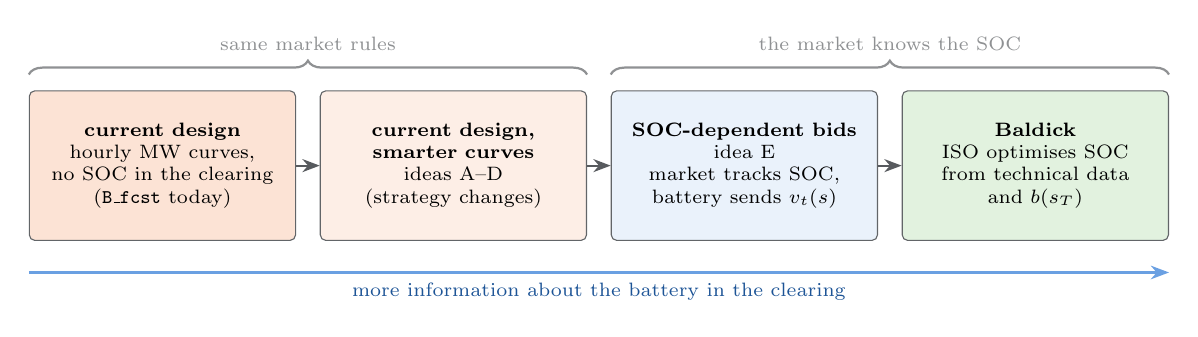
\begin{tikzpicture}[node distance=3mm,
  d/.style={box, text width=31mm, minimum height=19mm, font=\scriptsize}]
  \node[d, fill=lp] (cd) {\textbf{current design}\\hourly MW curves,\\no SOC in the clearing\\(\code{B\_fcst} today)};
  \node[d, fill=lp!60, right=of cd] (ad) {\textbf{current design,}\\\textbf{smarter curves}\\ideas A--D\\(strategy changes)};
  \node[d, fill=accent!10, right=of ad] (e) {\textbf{SOC-dependent bids}\\idea E\\market tracks SOC,\\battery sends $v_t(s)$};
  \node[d, fill=dat, right=of e] (b) {\textbf{Baldick}\\ISO optimises SOC\\from technical data\\and $b(s_T)$};
  \foreach \x/\y in {cd/ad, ad/e, e/b} \draw[arr] (\x) -- (\y);
  \draw[decorate, decoration={brace, amplitude=5pt}, thick, ink!50]
    ([yshift=2mm]cd.north west) -- ([yshift=2mm]ad.north east) node[midway, above=5pt, font=\scriptsize]{same market rules};
  \draw[decorate, decoration={brace, amplitude=5pt}, thick, ink!50]
    ([yshift=2mm]e.north west) -- ([yshift=2mm]b.north east) node[midway, above=5pt, font=\scriptsize]{the market knows the SOC};
  \draw[-{Stealth}, thick, accent!70] ([yshift=-4mm]cd.south west) -- ([yshift=-4mm]b.south east)
    node[midway, below, font=\scriptsize, text=accent!70!black]{more information about the battery in the clearing};
\end{tikzpicture}
\end{center}

% =====================================================================
\section{How idea C would build a curve}
% =====================================================================

\begin{center}
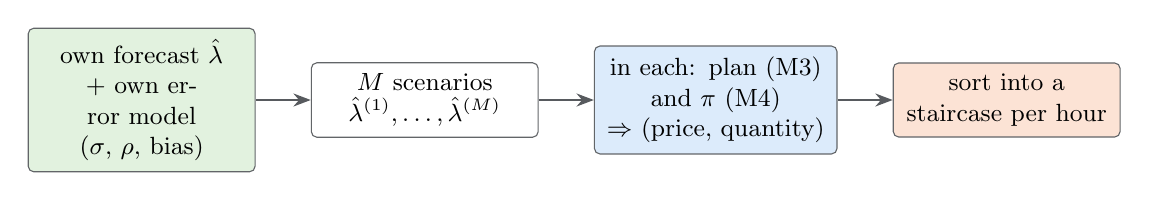
\begin{tikzpicture}[node distance=5mm and 7mm]
  \node[datbox, text width=26mm] (f) {own forecast $\lamhat$\\+ own error model\\($\sigma$, $\rho$, bias)};
  \node[box, right=of f, text width=26mm] (s) {$M$ scenarios\\$\lamhat^{(1)},\dots,\lamhat^{(M)}$};
  \node[box, fill=ex, right=of s, text width=28mm] (p) {in each: plan (M3)\\and $\pi$ (M4)\\$\Rightarrow$ (price, quantity)};
  \node[box, fill=lp, right=of p, text width=26mm] (c) {sort into a\\staircase per hour};
  \draw[arr] (f) -- (s); \draw[arr] (s) -- (p); \draw[arr] (p) -- (c);
\end{tikzpicture}
\end{center}
\begin{center}
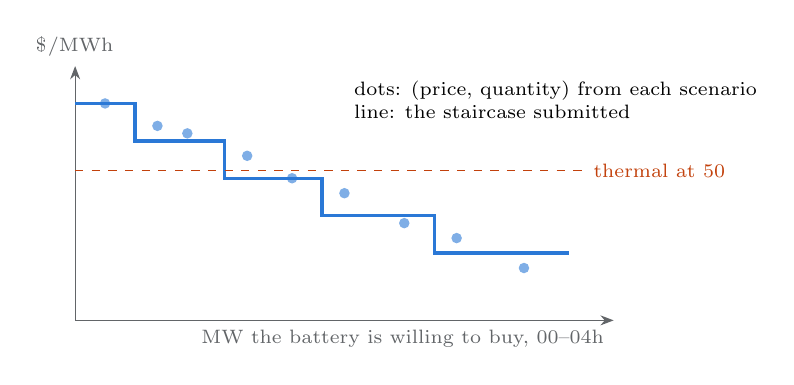
\begin{tikzpicture}[scale=0.95]
  \draw[-{Stealth}, ink!70] (0,0) -- (7.2,0) node[below left, font=\scriptsize]{MW the battery is willing to buy, 00--04h};
  \draw[-{Stealth}, ink!70] (0,0) -- (0,3.4) node[above, font=\scriptsize]{\$/MWh};
  \foreach \x/\y in {0.4/2.9, 1.1/2.6, 1.5/2.5, 2.3/2.2, 2.9/1.9, 3.6/1.7, 4.4/1.3, 5.1/1.1, 6.0/0.7} \fill[accent!60] (\x,\y) circle (2pt);
  \draw[very thick, accent] (0,2.9) -- (0.8,2.9) -- (0.8,2.4) -- (2.0,2.4) -- (2.0,1.9) -- (3.3,1.9) -- (3.3,1.4) -- (4.8,1.4) -- (4.8,0.9) -- (6.6,0.9);
  \draw[dashed, warn] (0,2.0) -- (6.8,2.0) node[right, font=\scriptsize, text=warn]{thermal at 50};
  \node[font=\scriptsize, align=left, anchor=west] at (3.6,2.95) {dots: (price, quantity) from each scenario\\line: the staircase submitted};
\end{tikzpicture}
\end{center}
{\small Illustration, not computed. Instead of one price for the whole spare capacity, the battery buys more
the cheaper the energy is, in proportion to how many of its scenarios say that purchase pays. Hypothesis: this
avoids the expensive ``buy from thermal at 00--04h'' regime ($\R_5$ in \code{regimes\_design.pdf}), because only a
small share of the curve sits above the thermal price.}

% =====================================================================
\section{Hypotheses and how to test them}
% =====================================================================

\begin{center}\small
\begin{tabularx}{\textwidth}{@{}l>{\raggedright\arraybackslash}X>{\raggedright\arraybackslash}p{4.6cm}@{}}
\toprule
Idea & Hypothesis & Test \\
\midrule
A, B & Do \emph{not} remove the 6.32\% perfect-price loss (they stay inside the plan's blind spot). & $\sigma=0$: loss $\approx6.32\%$ \\
C, D & Reduce the loss under forecast error, mainly by removing expensive regimes; no gain at $\sigma=0$. & paired comparison with \code{B\_fcst}, same error shapes, $\sigma\in\{1,\dots,20\}$ \\
E & Removes most of the perfect-price loss (the market sees the SOC); with D, also part of the forecast loss. & $\sigma=0$: loss $\to0$; then the $\sigma$ grid \\
\bottomrule
\end{tabularx}
\end{center}

\textbf{How every idea is scored.} A new bid family per idea (\code{B\_curve\_range}, \code{B\_curve\_dp},
\code{B\_curve\_scen}, \dots) returning more blocks per side; \code{market.clear\_hour} already accepts any number
of blocks, so clearing, real time and welfare (\code{runner.evaluate\_blocks}) are reused unchanged. Idea E needs
a new clearing variant that carries the SOC across hours (one multi-interval LP instead of six hourly ones).
It does not exist yet: the archived framework's \code{clearing.py} clears each hour independently and only
tracks the SOC afterwards; the root \code{CLAUDE.md} asked for an \code{soc\_enforced} switch, but it was never
built. \code{verify\_equivalence.build} already contains the SOC rows (A8)--(A10) that such a variant would reuse.

\begin{center}
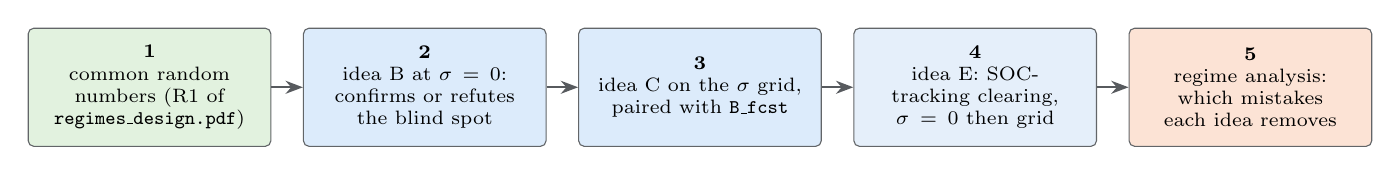
\begin{tikzpicture}[node distance=4mm,
  st/.style={box, text width=28mm, minimum height=15mm, font=\scriptsize}]
  \node[st, fill=dat] (s1) {\textbf{1}\\common random numbers (R1 of \code{regimes\_design.pdf})};
  \node[st, fill=ex, right=of s1] (s2) {\textbf{2}\\idea B at $\sigma=0$:\\confirms or refutes the blind spot};
  \node[st, fill=ex, right=of s2] (s3) {\textbf{3}\\idea C on the $\sigma$ grid,\\paired with \code{B\_fcst}};
  \node[st, fill=accent!12, right=of s3] (s4) {\textbf{4}\\idea E: SOC-tracking clearing, $\sigma=0$ then grid};
  \node[st, fill=lp, right=of s4] (s5) {\textbf{5}\\regime analysis: which mistakes each idea removes};
  \foreach \x/\y in {s1/s2, s2/s3, s3/s4, s4/s5} \draw[arr] (\x) -- (\y);
\end{tikzpicture}
\end{center}

% =====================================================================
\section{Questions to discuss}
% =====================================================================
\begin{enumerate}
  \item \textbf{Scope.} Is the thesis about \emph{market design} only (then A--D are a robustness check: ``the gap
    survives smarter bidding'') or also about \emph{how batteries should bid} in today's design (then C/D are a main
    result)? Possibly a question for the supervisors.
  \item \textbf{Idea E as a third design.} Comparing three designs (hourly curves / SOC-dependent bids / Baldick)
    instead of two would place the thesis in the current operator debate. Is it in scope, and which existing
    proposal should it follow?
  \item \textbf{Information assumptions.} Idea C assumes the battery knows its own error statistics; idea E assumes
    the market accepts an SOC-dependent value curve. Are both acceptable assumptions for the thesis?
  \item \textbf{Test system.} The coordination loss here is driven by exact ties of a 6-interval case. Should the
    curve ideas be evaluated directly on a larger, tie-free system (stage~1/3), where the picture may differ?
  \item \textbf{Order of work.} Proposed: common random numbers first, then the $\sigma=0$ test of B (one day of
    work) to confirm the diagnosis before investing in C--E.
\end{enumerate}

{\small\textbf{Numbers in \S1} come from the current code (\code{bids.bid\_star\_p}, prelimit rule,
\code{runner.evaluate\_blocks}, $\psi=10$), the same draw as \code{B\_star\_p} in the stage-0 notebook.
The figures in \S2 and \S4 are schematic illustrations, not computed results.}

\end{document}
